\header{
    \headtitle{Frère la Guillaumette} \label{frere-la-guillaumette}
    %
    
    \insertComment{Chanson de 1898 venant du Loiret (45).}{}
}

\enluminure{4}{\href{https://www.youtube.com/watch?v=7pVsCpIl3mM}{F}}{rère} la Guillaumette,
\\Quand tu rencontres une fillette,
\\Que fais-tu ?
\\Amen ! \textit{(le choeur)}
\\Je l'emmène dans ma chambrette,
\\Domi domino Domi dominette,
\\Je l'emmène dans ma chambrette, domino.
\\\\Frère la Guillaumette,
\\Quand tu rencontres une fillette,
\\Que tu l'emmènes dans ta chambrette,
\\Que fais-tu ?
\\Amen ! \textit{(le choeur)}
\\Je l'étends sur ma couchette
\\Domi domino Domi dominette,
\\Je l'étends sur ma couchette, domino.
\\\\Frère la Guillaumette,
\\Quand tu rencontres une fillette,
\\Que tu l'étends sur ta couchette,
\\Que fais-tu ?
\\Amen ! \textit{(le choeur)}
\\Je soulève ma chemisette
\\Domi domino Domi dominette,
\\Je soulève ma chemisette, domino.
\\\\Frère la Guillaumette,
\\Quand tu rencontres une fillette,
\\Que tu soulèves ta chemisette,
\\Que fais-tu ?
\\Amen ! \textit{(le choeur)}
\\Je déboutonne ma braguette
\\Domi domino Domi dominette,
\\Je déboutonne ma braguette, domino.
\breakpage
\textit{Avec la même construction :}
\\\\Je sors ma grosse bistouquette
\\J'me fais faire une p'tite branlette
\\J'me fais faire une p'tite sucette
\\Je lui écarte les gambettes
\\Je lui mets dans sa craquette
\\J'fais juter ma bistouquette
\\Je décharge dans sa craquette
\\Je tire une première crampette
\\Je tire une deuxième crampette
\\J'sens le bon Dieu dans mes roupettes
\\J'me fais faire une p'tite lichette
\\Je lui fais une p'tite minette
\\Je lui fous dans l'trou qui pète
\\Je r'tire ma p'tite bistouquette
\\Puis je la baise en levrette
\\J'lave la belle dans la cuvette
\\Je l'essuie dans la serviette
\\Je bois l'eau dans la cuvette
\\J'demande pardon à confesse
\\Je recherche une autre nonette
\\Je recommence l'historiette.
\\
\bigskip
\begin{center}
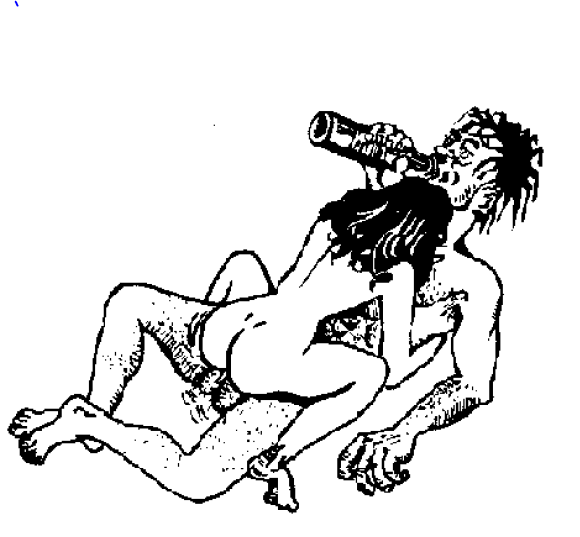
\includegraphics[width=0.7\textwidth]{images/image1.PNG}
\end{center}
\breakpage